\documentclass[12pt]{article}
\usepackage{graphicx}
\usepackage{url}
\usepackage{amsmath}
\usepackage{soul}
\usepackage{color}
\usepackage{tabularx}
\usepackage{makecell}
\setlength{\textwidth}{6.5in}
\setlength{\textheight}{9.9in}
\setlength{\oddsidemargin}{0.0in}
\setlength{\evensidemargin}{0.0in}
\setlength{\topmargin}{-2.5 cm}
\setlength{\parskip}{0.5\baselineskip} % space between paragraphs
\setlength{\parindent}{0 cm} % increase this if you like paragraphs to be indented

\pagestyle{empty}

\newcommand{\e}{\mathrm{e}}

% highlighting
\definecolor{hlcold}{rgb}{0.8,0.9,1.0}
\DeclareRobustCommand{\hlold}[1]{{\sethlcolor{hlcold}\hl{#1}}}
\definecolor{hlcnew}{rgb}{0.8,1.0,0.8}
\DeclareRobustCommand{\hlnew}[1]{{\sethlcolor{hlcnew}\hl{#1}}}
\definecolor{hlcedit}{rgb}{1.0,1.0,0.7}
\DeclareRobustCommand{\hledit}[1]{{\sethlcolor{hlcedit}\hl{#1}}}
\DeclareRobustCommand{\hldel}[1]{{\st{#1}}}

\begin{document}

\begin{center}

\bf{\LARGE
On the Relationship between Characteristics \\ and Parameters of Simple Pendulums
}

\rm{\large
Harry Chen\\
October 28, 2022
}

\end{center}


\section{Introduction}

The simple pendulum is one of the primary primitives in dynamics. While the experiments investigating the motion of a pendulum appear easy to conduct, the motion of a simple pendulum contains phenomena like harmonic motion and dissipation, and the relationship between characteristics like period and damping factor and parameters like string length and initial amplitude is the objective of this report. This report investigates the dependence between the period of a simple pendulum and the initial angle \hlnew{and length}, two models for the decay of the pendulum's amplitude over time\hlnew{, and the relationship between the pendulum's dissipation and length}.

In high school and college physics texts, the formula for the period of a pendulum is often given as: ~\cite{openstax-physics}

\begin{equation}
\label{equ:T}
T=2\pi\sqrt{\frac{L}{g}}
\end{equation}

where $L$ is the length of the pendulum and $g$ is the acceleration due to gravity. When $T$ is in seconds and $L$ is in meters, the formula $T=2\sqrt{L}$ is often used in practice. Equation \ref{equ:T} suggests the period of the pendulum is independent of the angle. \hldel{However, the experiment result shows that the period of the pendulum increases as the magnitude of the angle increases, and equation {\ref{equ:T}} only applies to small angles.} \hlnew{However, both theoretical and empirical evidences show that Equation {\ref{equ:T}} is only accurate for small angles.} For large angles, the following series expansion has been proposed: ~\cite{hyperphysics-pendl}

\begin{equation}
\label{equ:T1}
T=2\pi\sqrt{\frac{L}{g}}\left(1+\frac{1}{16}\theta^2+\mathrm{O}\left(\theta^4\right)\right)
\end{equation}

This equation suggests the period of a simple pendulum as a function of angle can be approximated by a parabola symmetrical about $\theta=0$. \hldel{The experiment result shows the parabola is not exactly symmetrical about $\theta=0$ and the dependency between period and angle is less significant compared to the prediction of Equation {\ref{equ:T1}}. This disagreement may be caused by the damping of the pendulum and other experimental errors.}

The motion of a pendulum with a damping force proportional to its velocity can be modeled by the following angle-time relationship: ~\cite{hyperphysics-oscda}

\begin{equation}
\label{equ:damped-osc}
\begin{aligned}
\theta(t)
&= \theta_{amp}(t) \cdot \theta_{osc}(t) \\
&= \theta_0 \e^{-t/\tau} \cdot \cos\left(\frac{2\pi}{T}t+\phi\right)
\end{aligned}
\end{equation}

where $\theta_0$ is the initial angle (or amplitude), $T$ is the period, $\tau$ is a coefficient related to damping, and $\phi$ is the phase shift. In the equation, the angle function $\theta(t)$ is the product of two functions of time: the amplitude function $\theta_{amp}(t)=\theta_0\e^{-t/\tau}$, and the oscillation function $\theta_{osc}(t)$. In engineering, the Q factor is often used to measure the damping of an oscillator. It is a dimensionless coefficient given by the following formula: ~\cite{wikipedia-q}

\begin{equation}
\label{equ:q}
Q=2\pi\frac{\tau}{T}
\end{equation}

In a perfectly exponentially decaying case, after $n$ periods, an oscillator has its amplitude decayed to $\e^{-2\pi n/Q}$ of its original amplitude. But in reality, the decay of the amplitude in a pendulum is rarely perfectly exponential. Hence, the following function term has been introduced, which is based on the assumption that the damping force is proportional to the square of the speed: ~\cite{quadratic-damp}

\begin{equation}
\label{equ:quadratic-damp}
\theta_{amp}(t) = \frac{\theta_0}{1+t/\tau}
\end{equation}

With the same $\theta_0$ and $\tau$, both amplitude functions have the same initial amplitude and decay rate. However, the quadratically-damped model (referred to as the \textit{rational model} in the remaining of this paper) decays slower as time proceeds, meaning it takes longer for the oscillator to damp to a certain amplitude. \hlnew{The damping is less significant for smaller angles and vice versa.} \hldel{This paper shows the rational model produces a better fit to experimental data and discusses this effect in Section {\ref{section:q}}.}

\hlnew{The effect of length on damping is more complex. A swinging pendulum experiences the drag of air, which is larger with a larger swinging speed. The pendulum also experiences the internal dissipation of the string. {\cite{pbm2001}} Let each dissipation be modeled by a power function $D=a'L^k$, and the total dissipation be the sum of the dissipation sources. Based on the Q factor being inversely proportional to the damping rate, I develop the following model for the Q factor vs. length relationship:}

\begin{equation}
\label{equ:q-length}
Q \sim \frac{1}{a_{air}L^{k_{air}}+a_{string}L^{k_{string}}}
\end{equation}

\hlnew{It is not difficult to predict $k_{air}$ with existing information. The speed of the mass on the pendulum is proportional to $L/T$, where $T\propto L^{1/2}$ according to Equation {\ref{equ:T}}. Therefore, the speed is proportional to $L^{1/2}$. Based on the assumption that air friction is proportional to the square of speed {\cite{quadratic-damp}}, I predict $k_{air}=1$, which means damping due to air resistance increases linearly as length increases and $a_{air}$ has unit $\mathrm{m}^{-1}$. Due to the conservation of energy, $a_{string}$ must be positive. A negative $k_{string}$ value indicates string damping decreases as length increases.}


\section{Methods and Procedures}

\begin{figure}[!htb]
\minipage{0.32\textwidth}
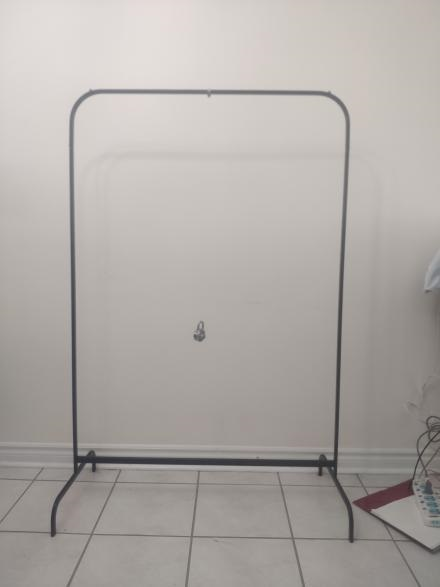
\includegraphics[width=\linewidth]{img-setup.jpg}
\caption{The overall pendulum setup}\label{fig:setup}
\endminipage\hfill
\minipage{0.32\textwidth}
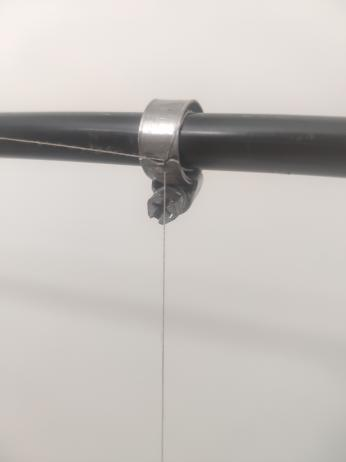
\includegraphics[width=\linewidth]{img-knot.jpg}
\caption{The pivot point of the pendulum}\label{fig:knot}
\endminipage\hfill
\minipage{0.32\textwidth}
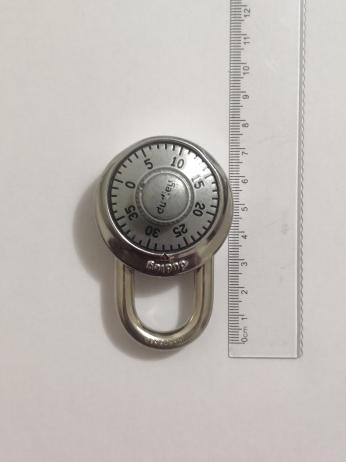
\includegraphics[width=\linewidth]{img-lock.jpg}
\caption{The lock as the mass}\label{fig:lock}
\endminipage
\end{figure}

The homemade pendulum used for experiments in this paper is made of a metal lock hanging on a thin sewing thread tied to the middle top of a black rectangular frame. The lock is chosen as the mass for its high density and thus has a higher resistance to air friction. The thread is chosen for its low mass and internal damping. These properties reduce the uncertainty caused by dissipation in the period-angle experiment. I chose a black rectangular frame to attach the string because it makes it easier to track the location of the lock related to the frame using computer vision software. During swinging, the lock oscillates in the air without making contact with a solid object.

In the period-angle experiment, the stretched length of the thread is $30\mathrm{cm}$, although the length of the pendulum used in the analysis is $35\mathrm{cm}\pm1\mathrm{cm}$ due to the consideration of the lock size. Trials are conducted for angles between $-90^\circ$ to $90^\circ$ with an increment of $20^\circ$. In each trial, the string is stretched and the lock is released from the specified angle, and one-twentieth of the time for the lock to complete 20 cycles is recorded as the period. Each trial is repeated 3 times. The angles are chosen for the convenience of measuring using a protractor with degree scales while skipping the zero angle, which has an undefined period. Angles are converted to radians in analysis. I measured the time of 20 cycles instead of 1 cycle to reduce the effect of human error on the period measurement. I started over the experiment after doing all trials once instead of repeating each angle trial 3 times in a row because I want to reduce the possible effects of previous trials on the current trial (ex. thread becoming loose.)

In the angle-time experiment, the lock is hanged on a thread with a rest length of $20\mathrm{cm}$ and released from an angle of $30^\circ$. Intuitively, a shorter string involves higher damping, which makes it faster for the amplitude of the pendulum to decay to a certain value. The angle is chosen to be small to reduce phase shift caused by the dependency of period and angle. A 60-second video is recorded and analyzed using OpenCV. \hlnew{The length of the thread used in data analysis is measured from motion capture data, which is longer than the rest length of the thread due to thread stretching and lock size.}

\hlnew{The period-length and Q factor-length experiments are conducted on selected rest string lengths with a procedure similar to the angle-time experiment. One change is made based on the results of the previous experiments: a larger initial angle ($40^\circ$) is chosen to increase damping since damping is an subject of this study. The length of the video recording is reduced to 40 seconds to comply with the larger angle, which results in a variable period and makes analysis more difficult. This is also based on the angle-time experiment showing data being less meaningful for $t>40\mathrm{s}$. (see {\ref{section:q}})}


\section{Results and Analysis}


\subsection{Period vs. Angle} \label{section:period-angle}

\begin{figure}[!ht]
\begin{center}
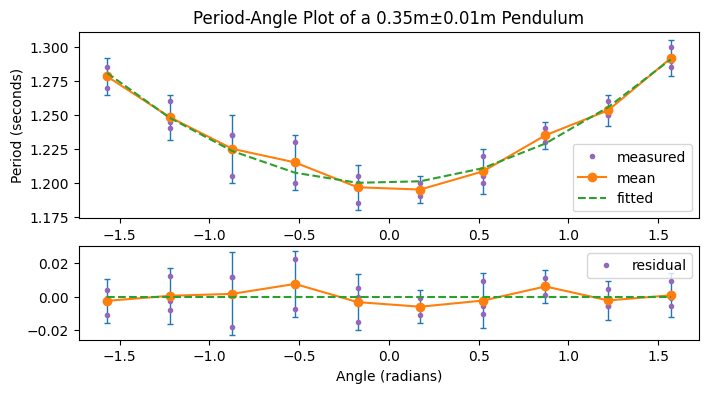
\includegraphics[width=0.7\textwidth]{period-angle.png}
\end{center}
\caption{Period-Angle Plot of a $0.35\mathrm{m}\pm0.01\mathrm{m}$ Pendulum}
\label{fig:period-angle}
\end{figure}

For the period-angle data, the period for an angle is taken as the mean of the three measures, and the uncertainty is taken as the minimum value required to cover all uncertainties of individual measurements. A parabolic function is used to fit the period vs. angle relationship. The curve of best fit has an equation $T(\theta)=T_0\left(1+b\theta+c\theta^2\right)$, where $T_0=1.20\mathrm{s}\pm0.02\mathrm{s}$, $b=0.003\pm0.001$, and $c=0.030\pm0.002$. The axis of symmetry of the parabola is $\theta=-\frac{b}{2c}=-0.05\pm0.02$.

As shown in Figure \ref{fig:period-angle}, the plot of the data has a roughly parabolic shape. The data is well-modeled by the parabolic function because all residuals are within the uncertainty interval. However, the value and uncertainty of its axis of symmetry suggest the parabola is not symmetrical about $\theta=0$. The residual has a slight, regular pattern roughly symmetrical about $\theta=0.2$. The $c$ value fitted from the data is about half of the magnitude as the value suggested by Equation \ref{equ:T1}.

The predicted period using the formula $T=2\sqrt{L}$ is $1.18\mathrm{s}\pm0.01\mathrm{s}$, merely touching the two lowest data points. Using the $T_0$ value and uncertainty generated by regression, the curve of best fit is within the uncertainty when $-0.5<\theta<0.4$. This suggests the dependence between the period and the angle can be ignored for $|\theta|<0.4$.


\subsection{Angle vs. Time} \label{section:angle-time}

\begin{figure}[!ht]
\begin{center}
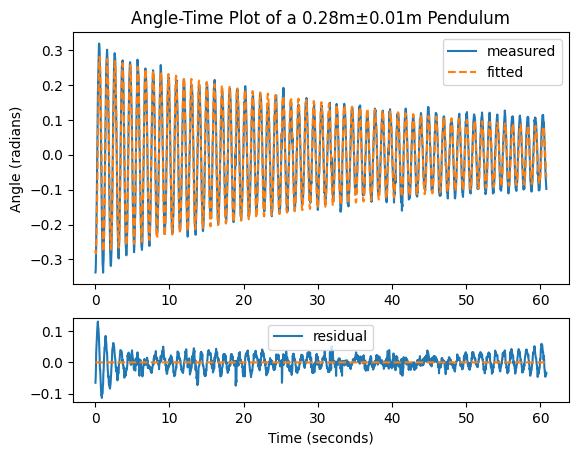
\includegraphics[width=0.7\textwidth]{angle-time.png}
\end{center}
\caption{Angle-Time Plot of a Simple Pendulum}
\label{fig:angle-time}
\end{figure}

The angle-time data is calculated from the lock positions tracked from the video. It contains about 1800 data points. The angles are subtracted from their mean to adjust bias during tracking caused by a skewed frame. Equation \ref{equ:damped-osc} is used to fit the data.

The curve of best fit has a $\tau$ value of $48.1\mathrm{s}\pm0.1\mathrm{s}$ and a period of $1.03091\mathrm{s}\pm0.00005\mathrm{s}$. As shown in Figure \ref{fig:angle-time}, it does not closely match the amplitude of the data: it underestimates the amplitude at the beginning at the end of the time interval and overestimates the amplitude at the middle of the time interval. The residual of the fit oscillates with a higher amplitude at the ends.


\subsection{Amplitude vs. Time} \label{section:amplitude-time}

\begin{figure}[!ht]
\begin{center}
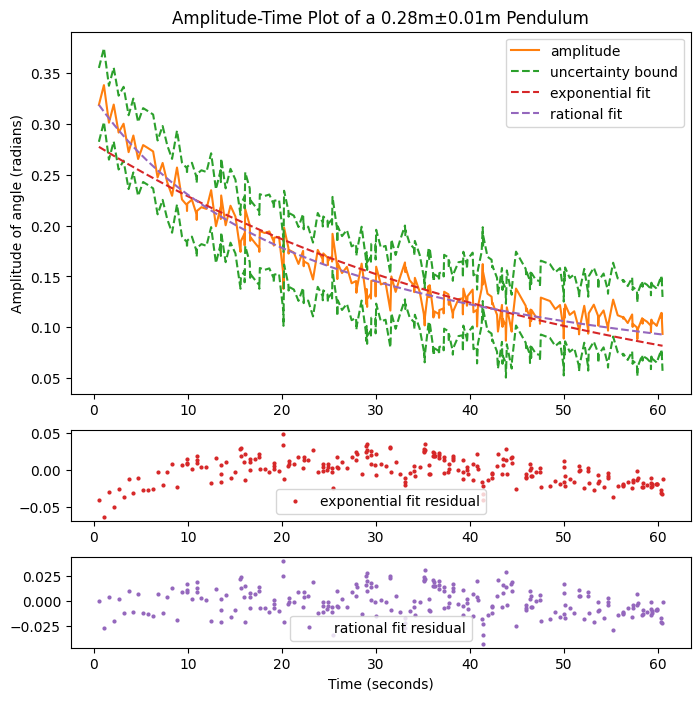
\includegraphics[width=0.7\textwidth]{amplitude-time.png}
\end{center}
\caption{Amplitude-Time Plot of a Simple Pendulum}
\label{fig:amplitude-time}
\end{figure}

The amplitude-time graph in Figure \ref{fig:amplitude-time} is generated by taking the absolute value of the extrema on the angle-time graph. It is noisy, primarily due to frame delay in the video skipping the actual extrema. But the noise is not a concern in this analysis because it is visually smaller than the uncertainties.

Overall, the plot is nonlinear with decaying amplitude and rate of change. Two decaying models introduced in the introduction are fit to the data. The exponential decay model has an initial amplitude of $0.281\mathrm{s}\pm0.004\mathrm{s}$ and a $\tau$ value of $49\mathrm{s}\pm1\mathrm{s}$. The rational decay model has an initial amplitude of $0.326\pm0.005\mathrm{s}$ and a $\tau$ value of $24.1\pm0.7s$. I don't consider the exponential decay model a good model because it does not closely fit the data, and the curve goes beyond the uncertainty interval at $t=0\mathrm{s}$. Also, there is a concave downward pattern in its residual. I consider the rational decay model to be appropriate for its close fit and no noticeable pattern in the residual. The advantage of the rational model over the exponential model is also seen from the coefficient of determination, where the rational model has $R^2=0.93$, higher than the exponential model's $R^2=0.88$.


\subsection{Discussion on the Q Factor} \label{section:q}

The Q factor of the oscillation is calculated using Equation \ref{equ:q}. Using $\tau$ value obtained from fitting the exponential model, the $Q$ is calculated to be $298\pm6$. Using $\tau$ value obtained from fitting the rational model, the initial $Q$ is calculated to be $147\pm4$. The exponential model has a $Q$ value about twice as high as that of the exponential model. However, since the uncertainty and residual showed that the exponential model is not an appropriate fit, the Q factor may not be constant over time, and the Q factor calculated from the exponential fit may be an average of $Q$ values throughout the time interval.

Using the formula $\theta_f/\theta_i=\e^{-2\pi n/Q}$, the Q factor during a shorter time interval can be determined. \hlnew{Table {\ref{table:q-change}} presents Q factors calculated based on the change of amplitude over selected time intervals with amplitude data manually read from Figure {\ref{fig:amplitude-time}}.}

\begin{table}[h]
\begin{tabularx}{\textwidth}{ |l|l|l|X| }
\hline
Time range &
Amplitude range &
Q factor &
Comment
\\ \hline
$0\mathrm{s}$ to $10\mathrm{s}$ &
$0.32\pm0.01$ to $0.21\pm0.01$ &
$150\pm20$ &
Matches the Q factor calculated from the rational fit ($147\pm4$)
\\ \hline
$10\mathrm{s}$ to $20\mathrm{s}$ &
$0.21\pm0.01$ to $0.17\pm0.01$ &
$290\pm80$ &
Matches the Q factor calculated from the exponential fit ($298\pm6$)
\\ \hline
$20\mathrm{s}$ to $40\mathrm{s}$ &
$0.17\pm0.01$ to $0.13\pm0.01$ &
$500\pm100$ &
Exceeds the Q factor of the exponential model
\\ \hline
\end{tabularx}
\caption{\hlnew{Q factors based on amplitude changes in selected time ranges}}
\label{table:q-change}
\end{table}

\hldel{Consider the interval from $t=0\mathrm{s}$ to $t=10\mathrm{s}$: there are $9.7002\pm0.0004$ periods in this interval, the amplitudes at the endpoints are respectively $0.32\pm0.01$ and $0.21\pm0.01$, the Q factor is calculated to be $145\pm16$, matching the Q factor calculated from the rational model. At $t=10\mathrm{s}$ and $t=20\mathrm{s}$, the amplitudes are $0.21\pm0.01$ and $0.17\pm0.01$, the Q factor calculated in between is $290\pm80$, matching the Q factor of the exponential model. Between $t=20\mathrm{s}$ and $t=40\mathrm{s}$, the Q factor is $450\pm130$, exceeding the Q factor of the exponential model. This shows the Q factor increases as time increases, and fitting the rational model captures the Q factor near the start of the oscillation.}

\hlnew{It is clear that the Q factor increases as time increases. The Q factor on the time range with the smallest $t$ matches the Q factor calculated from the parameters of the rational fit, indicating the Q factor based on the rational fit captures the start of the oscillation. The Q factor based on the exponential fit matches the Q factor on a time interval in the middle, meaning it captures an average of all Q factors in the oscillation. As time increases, the local Q factor increases beyond the Q factor based on both fits.}

% https://www.desmos.com/calculator/fb5ay3gfny


\subsection{Period vs. Length} \label{section:period-length}

\begin{figure}[!htb]
\minipage{0.55\textwidth}
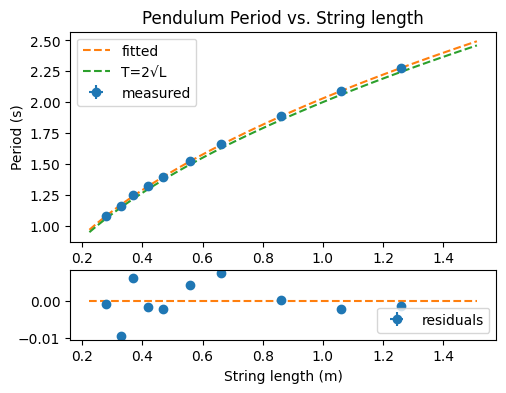
\includegraphics[width=\linewidth]{period-length.png}
\caption{Period-length plot of a single pendulum}\label{fig:period-length}
\endminipage\hfill
\minipage{0.4\textwidth}
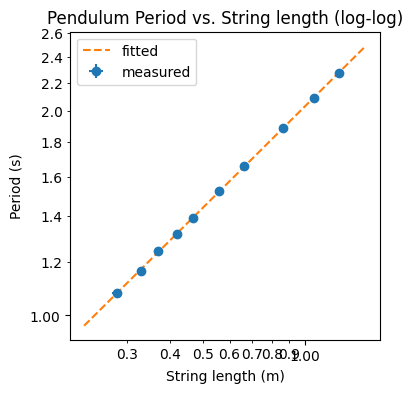
\includegraphics[width=\linewidth]{period-length-log.png}
\caption{The same period-length plot on logarithmic axes}\label{fig:period-length-log}
\endminipage
\end{figure}

\hlnew{The period-length data collected from the experiment is fitted to a power function $T=aL^k$. Equation {\ref{equ:T}} predicted that when $T$ is in seconds and $L$ is in meters, the values of $a$ and $k$ are respectively $2$ and $0.5$. The result of the fitting finds that $a=2.030\pm0.002$ and $k=0.497\pm0.002$. These values are very close to the prediction but do not equal based on uncertainty.}

\hlnew{Visually, points on linear-scale plot Figure {\ref{fig:period-length}} have barely noticeable deviation from the line of best fit, and the residuals do not have a pattern. When plotted on logarithmic axes (Figure {\ref{fig:period-length-log}}), the points are arranged on a straight line with a coefficient of determination $R^2=0.9998$. This means the period-length relationship is well-modeled by a power function.}

\hlnew{In Figure {\ref{fig:period-length}}, the curve of best fit is slightly higher than the predicted curve. I consider the cause of this deviation to be the angle in the pendulum. Based on the result in {\ref{section:angle-time}} that a pendulum's period increases as the angle increases, and considering in the experiment the initial angles were large ($\approx 0.7$), I consider it normal that the measured period is higher than an angle-independent predicted period.}


\subsection{Q Factor vs. String Length} \label{section:q-length}

\begin{figure}[!ht]
\begin{center}
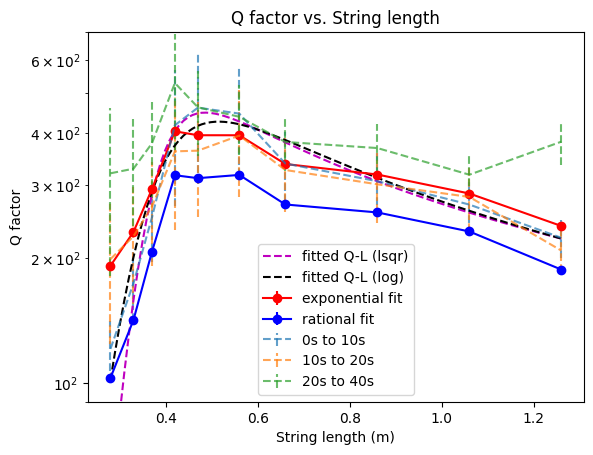
\includegraphics[width=0.8\textwidth]{q-length.png}
\end{center}
\caption{Q factor$-$length plot of a simple pendulum}
\label{fig:q-length}
\end{figure}

\hlnew{For the oscillation with each length, five Q factors are calculated: two are from parameters of exponential and rational fits, and three are calculated on different time intervals.}

\hlnew{As shown in Figure {\ref{fig:q-length}}, as the string length increases, the Q factor increases until reaching a peak at a length between $0.4\mathrm{m}$ and $0.6\mathrm{m}$ and then declines steadily. The shape of the plot of the Q factor calculated from the exponential and rational fits roughly match, except the rational fit results are lower than the exponential fit results, which has been discussed in {\ref{section:q}}.}

\hlnew{The Q factors between $t=10\mathrm{s}$ and $t=20\mathrm{s}$ match well with the exponential fit Q factors, and the Q factors between $t=20\mathrm{s}$ and $t=40\mathrm{s}$ are greater than the exponential fit factors, although some are overlapping with consideration of uncertainty. These resemble the results in Section {\ref{section:amplitude-time}}. In contrast to Section {\ref{section:amplitude-time}}'s result, the Q factor approaches exponential fit Q factors as the string length increases. Although they merely touch the rational fit Q factors with the consideration of uncertainties, their values are very close to exponential fit Q values for $L>0.6\mathrm{m}$, meaning the rational model captures the initial damping less accurately than the exponential model does for large lengths.}

\hlnew{I choose to fit equation {\ref{equ:q-length}} to the Q factor between $0\mathrm{s}$ and $10\mathrm{s}$ to minimize the effect of angle change on damping rate. Lengths used in fitting are in meters. Inspired by the log mode on the Desmos graphing calculator {\cite{desmos-log-mode}}, I take a logarithm before applying least squares fitting to reduce the nonlinearity of data, and I compare it with a simple least squares fitting. Overall, log mode produces a better result because the curve of best fit meets all data points with uncertainty. The simple least squares fitting fails to meet Q factors on small lengths. The parameters of regression are given in Table {\ref{table:q-length-fit}}.}

\begin{table}[h]
\begin{tabularx}{\textwidth}{ |X|l|l|l|l| }
\hline
Fitting mode &
$a_{air}$ & $k_{air}$ &
$a_{string}$ & $k_{string}$
\\ \hline
Least squares &
$0.0037\pm0.0002$ & $0.8\pm0.2$ &
$0.6\times10^{-6}\pm1.4\times10^{-6}$ & $-8\pm2$
\\ \hline
Log mode &
$0.0036\pm0.0002$ & $0.9\pm0.2$ &
$1.0\times10^{-5}\pm1.5\times10^{-5}$ & $-5\pm1$
\\ \hline
\end{tabularx}
\caption{\hlnew{Parameters of Q factor$-$length fitting. Note that $a_{string}$ is reported to an extra significant digit.}}
\label{table:q-length-fit}
\end{table}

\hlnew{The two fits have consistent air friction parameters and confirm the prediction that $k_{air}=1$. $k_{string}$ values are negative, indicating a negative correlation between string damping and length. However, the string damping in the two fits is inconsistent, where the log fit produces a higher leading coefficient and a lower exponent magnitude. Based on uncertainty, $a_{string}$ can be negative, which is impossible due to the conservation of energy. I consider the cause of this issue to be numerical instability in fitting, and therefore parameters related to string damping are unreliable.}


\section{Conclusion}

The period-angle experiment shows the period of a pendulum is dependent on the angle and increases as the magnitude of the angle increases, and their relationship can be well-modeled by a parabolic function. While there is a regular pattern in the residual when fitted to a parabola, considering they are small and are within the data uncertainty, I account for the cause of this pattern for experimental dependencies. The formula $T=2\sqrt{L}$ applies for small $\theta$, or, $|\theta|<0.4$. \hlnew{The actual period is larger than the period predicted by the equation for large $\theta$ values.} Due to the damping of the pendulum angle in the experiment and other uncertainties, it is not sufficient to show whether the period-angle relationship resembles or deviates from Equation \ref{equ:T1}. Future experiments may be conducted with time measured over a fewer number of periods to reduce the effect of damping on the data.

The amplitude-time data shows the amplitude of the pendulum decays in a nonlinear pattern, which is more accurately modeled by a rational function than an exponentially decaying function. The Q factor calculated from the regression parameters of the rational model matches the Q factor calculated from the decay of the amplitude near the start of the curve. The latter Q factor decreases as the motion progresses.

\hlnew{Two main sources of dissipation of the pendulum are air resistance and string damping. Air resistance is proportional to the square of the pendulum's speed, which increases as the pendulum length increases. Empirically, the damping of the string decreases as length increases. Considering both damping sources, the pendulum studied in this experiment reaches a maximum Q factor at $L=0.5\mathrm{m}\pm0.1\mathrm{m}$ and decreases when $L$ is higher or lower. However, due to numerical issues in fitting, it is not sufficient to have an educated conclusion on the relationship between damping and string length.}

There are numerous sources of uncertainty in this experiment. One observation to note is that the pendulum does not always swing "back and forth": the motion gradually turned into an elliptical motion in 3D, which deviates from the assumption that the weight moves on a two-dimensional plane. A factor contributing to this error is the thread is simply tied to the top of the frame and able to swing freely in different directions. The elliptical motion may be reduced by restricting the motion of the thread by placing a rigid plate near the pivot point. The most significant error in \hldel{this experiment} \hlnew{period-angle and angle-time experiments} is very likely the frame. As shown in Figure \ref{fig:setup}, the vertical columns of the frame are not completely straight, and the frame moved as the pendulum swan, making the pivot point of the pendulum movable. \hldel{This can be improved in the future by using a more rigid frame.} \hlnew{This was improved in variable length trials by clamping the frame between two desks.} Human error is also responsible for uncertainty in the experiment. It took several seconds before I pressed the camera button after I released the pendulum, which allowed damping to occur during this time. Although I released the pendulum from $30^\circ$ ($0.52$ radians), the data suggests the pendulum has an initial amplitude of $0.32\pm0.01$ radians, which is considerably less than the intended angle. This can be resolved by collaborating with another person or using automated equipment.


%\newpage
\bibliographystyle{IEEEtran}
\bibliography{refs}


\newpage
\appendix


\section{Data for Variable Angle Trials} \label{appendix:period-angle}

\hlnew{The following table presents measurements of periods on different angles. Angles are in radians and period measurements are in seconds with an uncertainty of $0.005\mathrm{s}$. These data are used for plotting Figure {\ref{fig:period-angle}} and analysis in Section {\ref{section:period-angle}}.}

\begin{table}[h]
\begin{tabularx}{\textwidth}{ |X|c|c|c|c|c|c|c|c|c|c| }
\hline
Initial Angle &
-1.57&-1.22&-0.87&-0.52&-0.17&0.17&0.52&0.87&1.22&1.57
\\ \hline
Trial 1 &
1.270&1.240&1.205&1.200&1.185&1.190&1.205&1.240&1.250&1.285
\\ \hline
Trial 2 &
1.280&1.245&1.235&1.215&1.200&1.200&1.200&1.230&1.260&1.290
\\ \hline
Trial 3 &
1.285&1.260&1.235&1.230&1.205&1.195&1.220&1.235&1.250&1.300
\\ \hline
\end{tabularx}
\caption{\hlnew{Measurements of periods on various angles}}
\label{table:period-angle}
\end{table}


\section{Data for Variable Length Trials} \label{appendix:variable-length}

\hlnew{Key values are calculated from curve fitting parameters from data in variable length trials. These include the measured length, the period, and Q factors calculated using different methods, which are used for analysis in Section {\ref{section:period-length}} and Section {\ref{section:q-length}}.}

\begin{table}[h]
\begin{tabularx}{\textwidth}{ |l|X|l|l|l|l|l| }
\hline
\makecell[l]{Measured\\length (m)} &
Period (s) &
\makecell[l]{Q\\(expon-\\ential fit)} &
\makecell[l]{Q\\(rational\\fit)} &
\makecell[l]{Q\\(0s-10s)} &
\makecell[l]{Q\\(10s-20s)} &
\makecell[l]{Q\\(20s-40s)}
\\ \hline
0.28±0.01 &
1.07821±0.00008 &
191±1 & 102.7±0.3 & 120±20 & 200±70 & 300±100
\\ \hline
0.33±0.01 &
1.16121±0.00009 &
231±1 & 141.7±0.3 & 170±30 & 230±70 & 300±100
\\ \hline
0.37±0.01 &
1.24532±0.00009 &
293±1 & 206.6±0.1 & 250±50 & 270±70 & 400±100
\\ \hline
0.42±0.01 &
1.31807±0.00006 &
403.7±0.9 & 316.3±0.7 & 400±200 & 400±100 & 500±200
\\ \hline
0.47±0.01 &
1.39318±0.00006 &
395.0±0.7 & 311.2±0.4 & 500±200 & 400±100 & 500±100
\\ \hline
0.56±0.01 &
1.52664±0.00006 &
394.9±0.5 & 316.9±0.2 & 400±100 & 400±100 & 440±80
\\ \hline
0.66±0.01 &
1.65924±0.00008 &
336.7±0.5 & 268.9±0.2 & 340±60 & 330±70 & 380±60
\\ \hline
0.86±0.01 &
1.88390±0.00006 &
317.6±0.5 & 257.3±0.1 & 300±50 & 300±60 & 370±50
\\ \hline
1.06±0.01 &
2.08767±0.00006 &
285.8±0.4 & 231.5±0.1 & 270±40 & 280±50 & 320±40
\\ \hline
1.26±0.01 &
2.27583±0.00009 &
238.7±0.9 & 187.4±0.6 & 220±20 & 200±20 & 380±50
\\ \hline
\end{tabularx}
\caption{\hlnew{Measurements of lengths, periods, and Q factors on variable length trials}}
\label{table:variable-length}
\end{table}

\end{document}


